
One avenue for testing quartic gauge boson interactions is through
inclusive tri-boson production: $pp\ to VV^{\prime}V^{\prime\prime}$
for $V= \gamma, W, Z$.  Using the Run 1 data sample, the triply heavy
such channels ($WWW, WWZ, WZZ, ZZZ$) are not accessible anywhere near
SM rates, due to their small 8 TeV cross sections and large
multi-lepton backgrounds. The photonic channels do not suffer as much
from these problems, and sensitivity is at or near SM rates in Run 1. 

ATLAS $W\gamma\gamma$~\cite{Aad:2015uqa}
\begin{figure}[p]
    \centering
    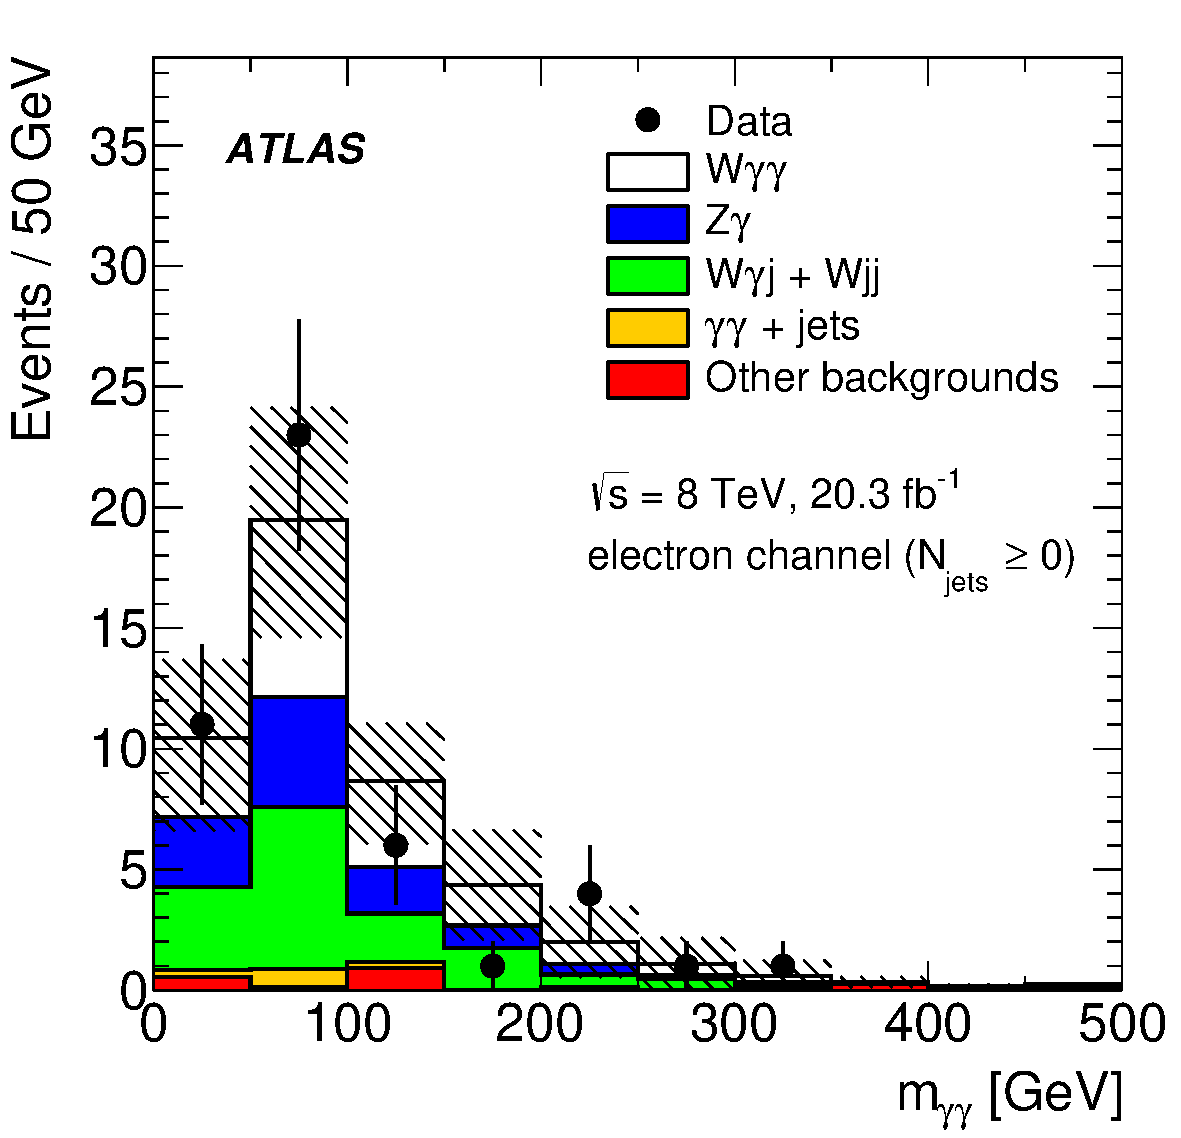
\includegraphics[width=0.45\textwidth]{figures/ss-inclboson-triboson-wgg-ele-atlas8tev.pdf}
    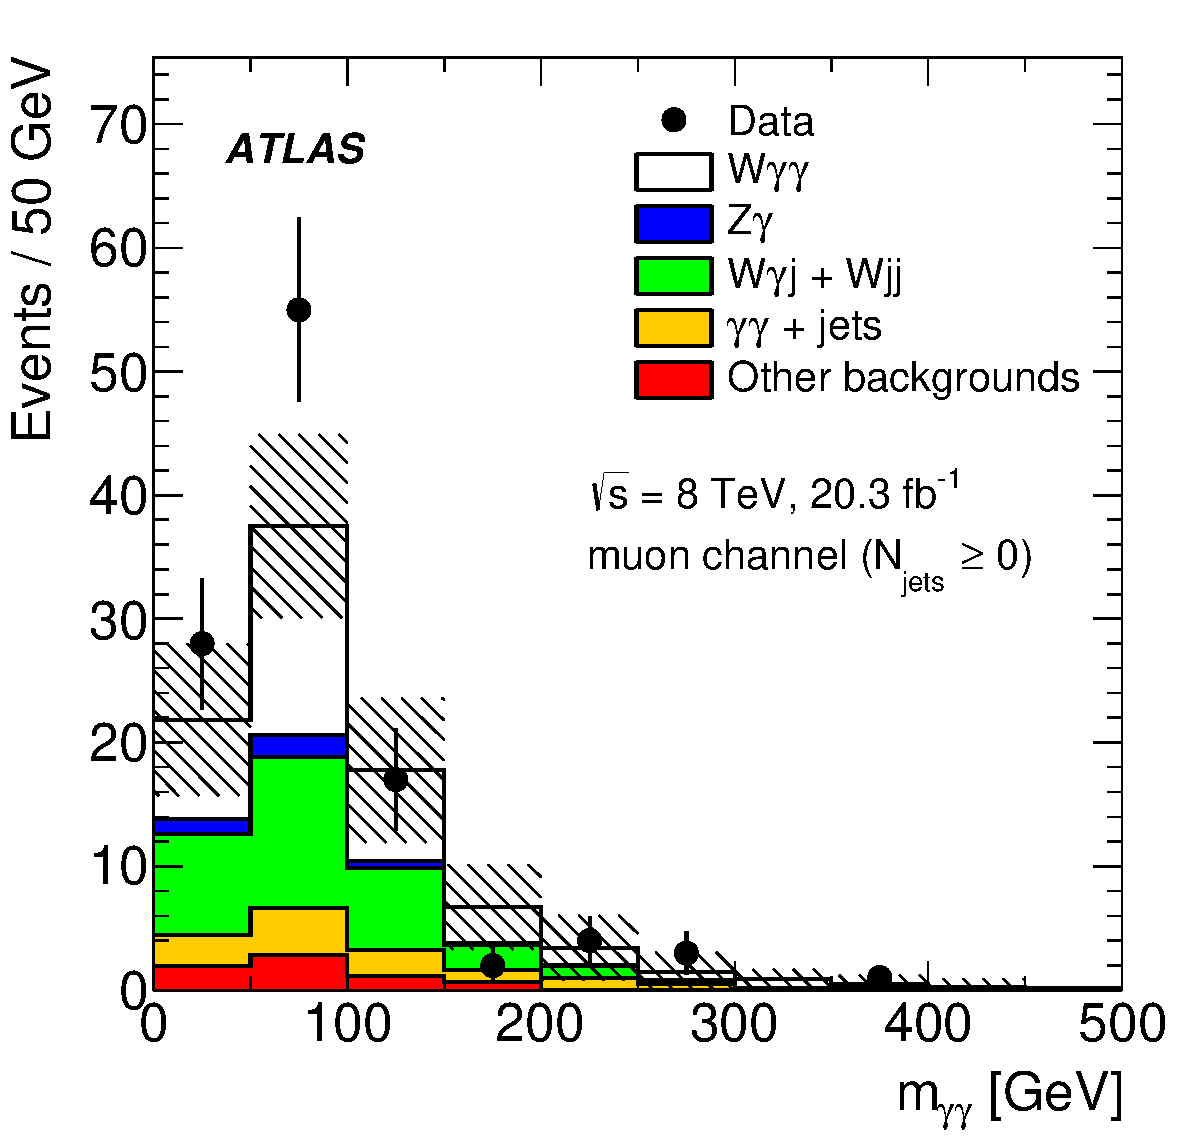
\includegraphics[width=0.45\textwidth]{figures/ss-inclboson-triboson-wgg-mu-atlas8tev.pdf}
    \caption{}
    \label{fig:ss-inclboson-triboson-wgg-atlas8tev}
\end{figure}


CMS WVgamma 8 \TeV~\cite{Chatrchyan:2014bza}

\begin{figure}[p]
    \centering
    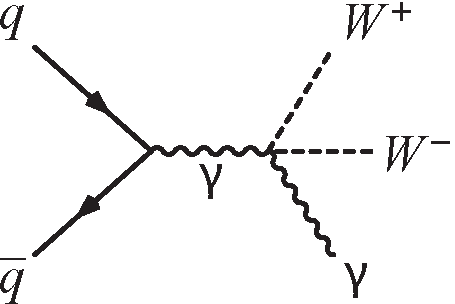
\includegraphics[width=0.45\textwidth]{figures/ss-inclboson-triboson-wvg-diagram1.pdf}
    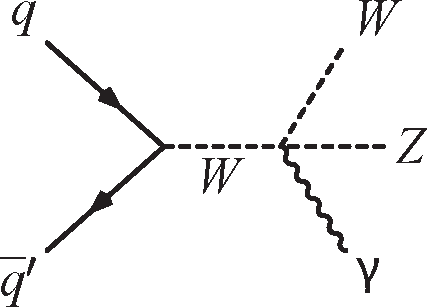
\includegraphics[width=0.45\textwidth]{figures/ss-inclboson-triboson-wvg-diagram2.pdf}
    \caption{}
    \label{fig:ss-inclboson-triboson-wvg-diagrams}
\end{figure}
\begin{figure}[p]
    \centering
    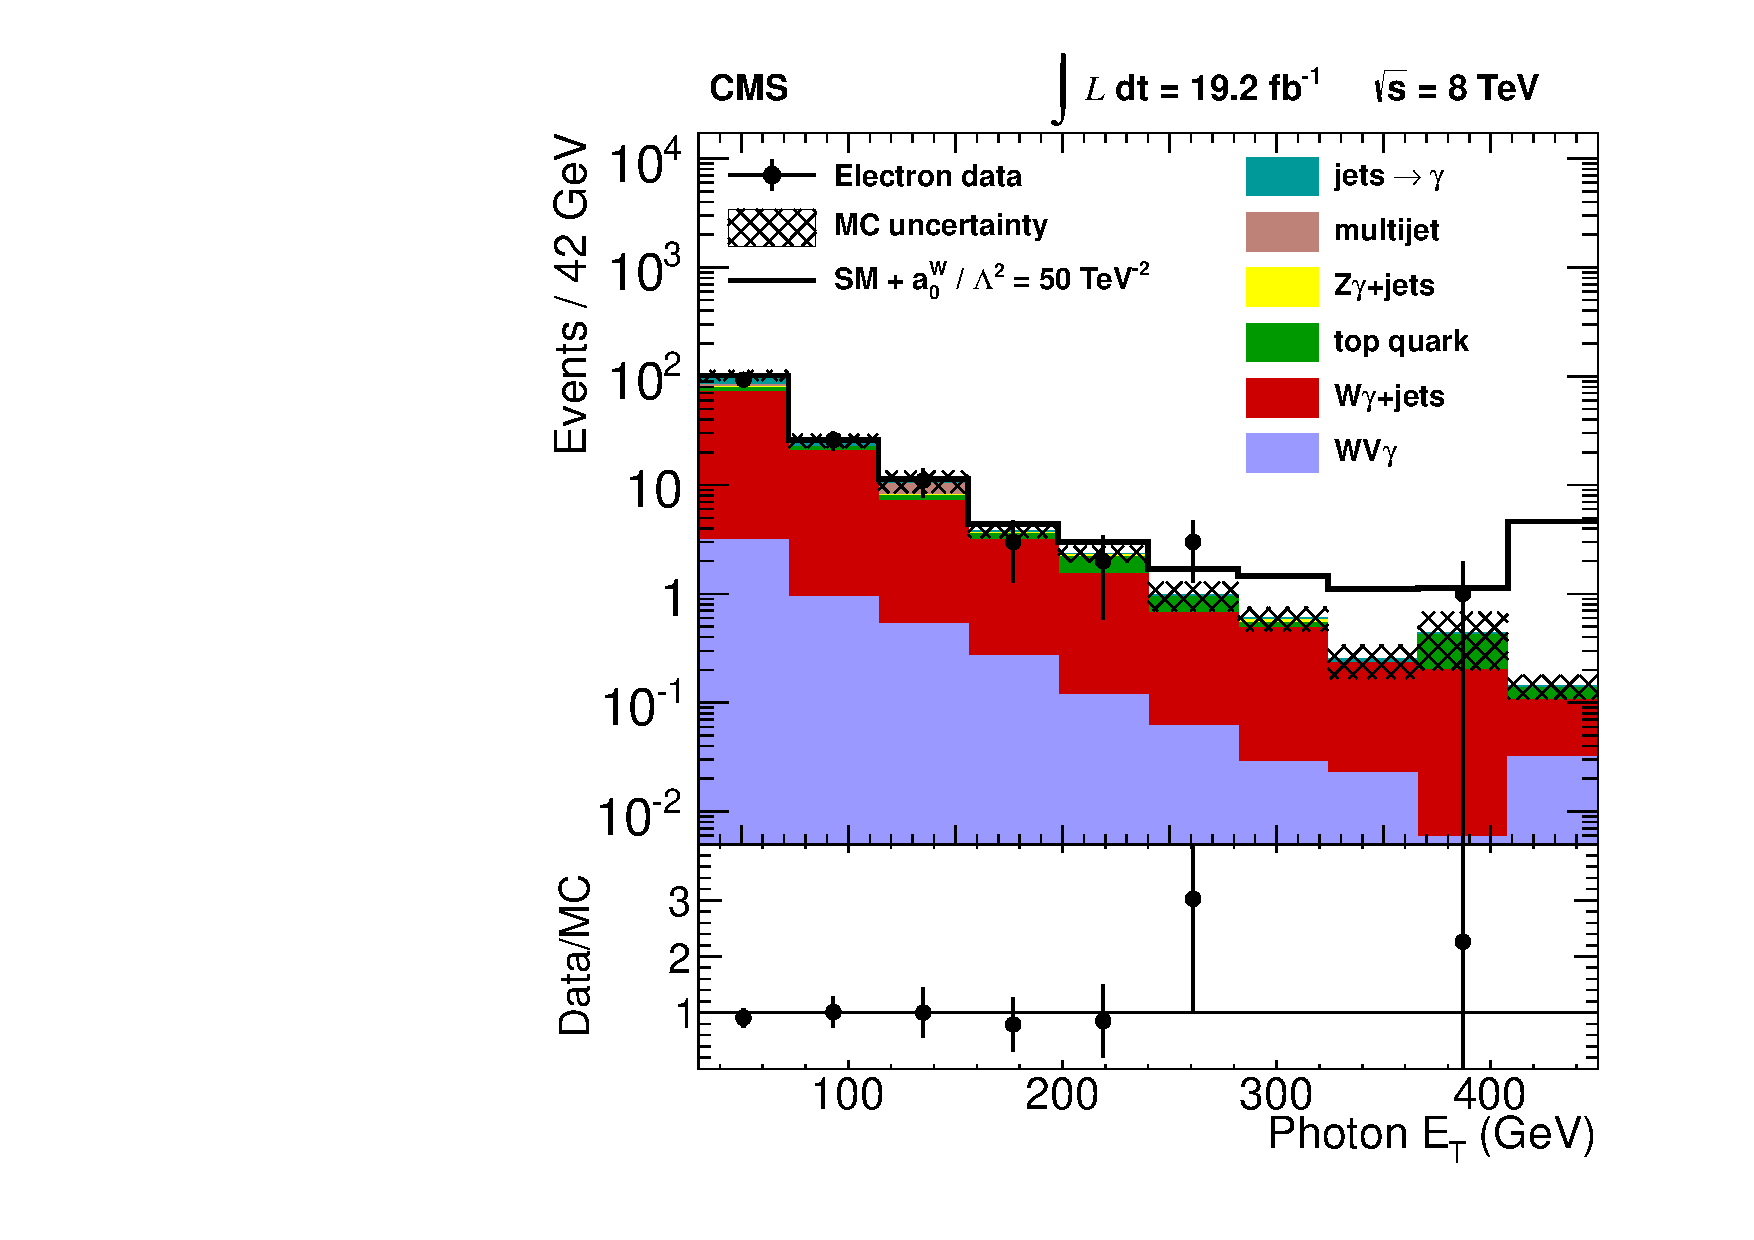
\includegraphics[width=0.45\textwidth]{figures/ss-inclboson-triboson-wvg-ele-cms8tev.pdf}
    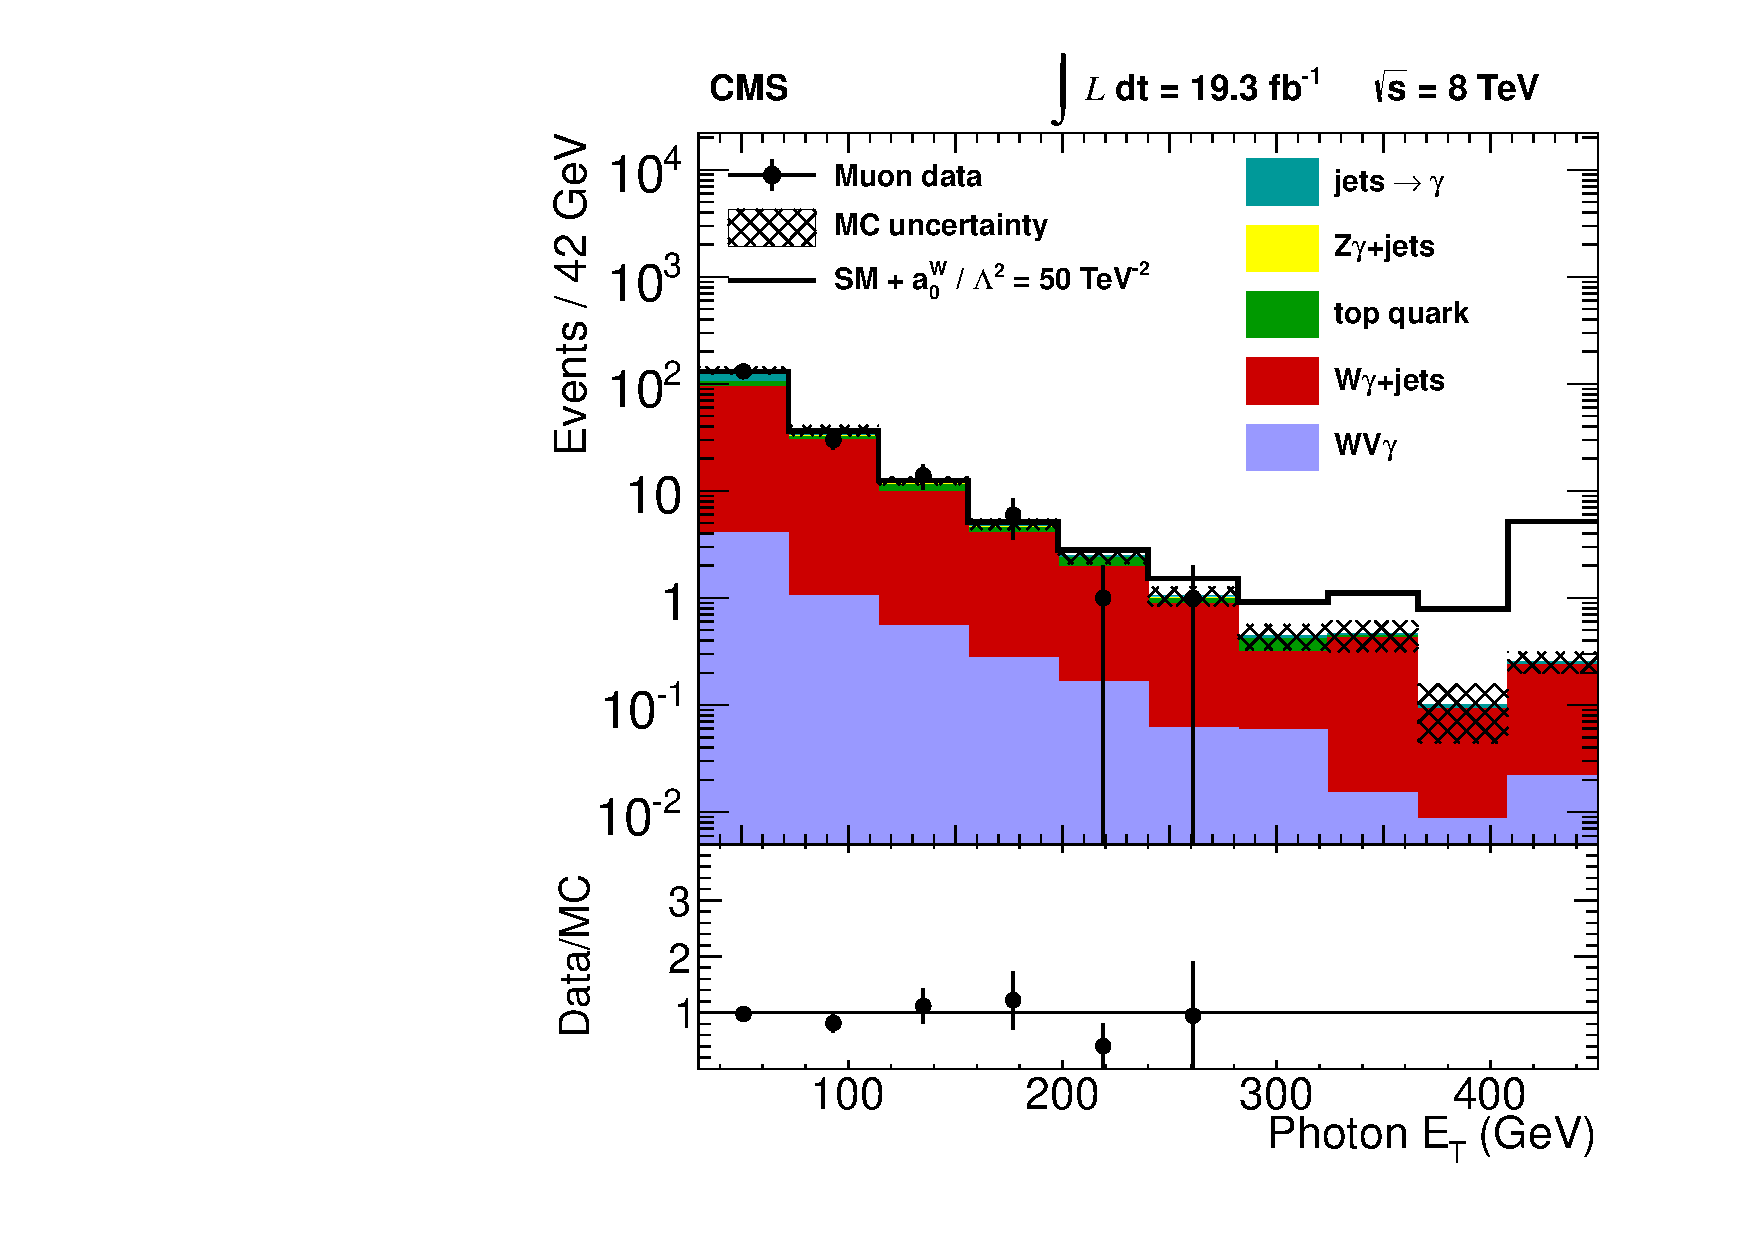
\includegraphics[width=0.45\textwidth]{figures/ss-inclboson-triboson-wvg-mu-cms8tev.pdf}
    \caption{}
    \label{fig:ss-inclboson-triboson-wvg-cms8tev}
\end{figure}
